
\documentclass{beamer}
\usetheme{PaloAlto} %was Warsaw, Singapore, PaloAlto, Ilmenau, Boadilla
% see http://www.pletscher.org/writings/latex/beamerthemes.php
\usepackage{verbatim} %for comments
\usepackage[english]{babel}
\usepackage[latin1]{inputenc}
\usepackage{amsmath}
\usepackage{mathrsfs}
\usepackage{epsfig}
\usepackage{epic}
\usepackage{amsmath}
\usepackage{amsfonts}
\usepackage{amssymb}
\usepackage{latexsym}
\usepackage{multirow}
\usepackage{verbatim}
%\usepackage{algorithm}


\AtBeginSection[]
{
  \begin{frame}<beamer>
    \frametitle{Volume and Integration}
    \tableofcontents[currentsection,currentsubsection]
  \end{frame}
}


\begin{document}

\title{Latte Valuations: Volume and Integration}
\author{}
\date{\today}

\frame{\titlepage}

\section{Volume}




\frame{
\frametitle{Two Flavors}
Latte can compute normalized volumes of polytopes using two different methods:
\begin{enumerate}
\pause
\item The Triangulation Method: Triangulate the polytope into simplices, then use the determinant to find the volume of each simplex.
\pause
\item The Lawrence Method: Triangulate every vertex tangent-cone into simplicial cones and then use a volume formula by Jim Lawrence.
\end{enumerate}
}%frame

\subsection{Triangulation Algorithm}

\frame{
\frametitle{Volume of a square}
\begin{center}
\resizebox{1.5in}{!}{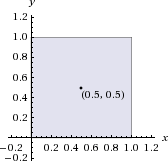
\includegraphics[]{img/unitSquare.png}}
\end{center}
Take the unit square centred at $(1/2, 1/2)$ above; after triangulation, we have two triangles: $\left\lbrace   (0, 0), (1, 0), (1, 1)\right\rbrace$ and $\left\lbrace  (0, 0), (0, 1), (1, 1)\right\rbrace$. Summing the determinant of tiangles' rays and dividing by two give the volume as 1.
}%frame


\frame{
\frametitle{Volume of a square}
\begin{center}
\resizebox{1.5in}{!}{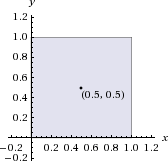
\includegraphics[]{img/unitSquare.png}}
\end{center}
In general, if $\left\lbrace (v_{0i}, v_{1i}, \ldots, v_{di})\right\rbrace  = T_i$ forms a d-simplex such that
the family $\left\lbrace T_1, \ldots, T_k \right\rbrace = \mathcal{T}$ is a triangulation of a d-Polytope, then the volume is given by:

$$
\sum_{T_i \in \mathcal{T}} |\det ( v_{1i} - v_{0i}, \ldots, v_{di} - v_{0i})| / d!
$$
}%frame

\subsection{Triangulation Example}
\frame{
\frametitle{Volume of a square}
For the first step in latte, we need create a file containing he hyperplanes that define the polytope. If $P = \left\lbrace x : Ax < b \right\rbrace$ for some $m \times n$ matrix $A$, then the input file will have the form:

$$
\begin{array}{l l}
 m & n + 1 \\
 \multicolumn{2}{l}{0 \leq b_{i} - a_{i}} \\

\end{array}
$$

where $b_{i}$ is the $i^{th}$ entry of b and $a_i$ is the $i^{th}$ row of $A$.
}%frame


\frame{
\frametitle{Volume of a square}
For our square, its defining hyperplanes are 
$$0 \leq x \leq 1, 0 \leq y \leq 1$$
and so we create a file that contains

\begin{block}<+->{square.latte}
	\begin{tabular}{rrr}
	4 &3 & \\
	0 &1 &0 \\
	1 &-1 &0 \\
	0 &0 &1 \\
	1 &0 &-1 \\
	\end{tabular}
\end{block}

}%frame



\frame{
\frametitle{Volume of a square}
Finally, the command we need is 

\begin{block}<+->{Command:}
./ValuationComputation  --valuation=volume --triangulate square.latte
\end{block}

\begin{block}<+->{Output:}
Volume (using the triangulation-determinant method) \\*
Answer: 1 (as a fraction) \\*
Decimal: 1 \\*
Time: 0.00 sec
\end{block}

}%frame

\subsection{Lawrence Algorithm}


\frame{
\frametitle{Volume of a Square}

Take the same unit square the Lawrence formula gives the volume in terms of the vertices and rays of every tangent cone. If the tangent cones are not simplicial, they must be first triangulated. For our square, the simplicial tangent cones are:

\begin{center}
\begin{tabular}{|c|c|}
	\hline
	Vertex & Rays \\
	\hline
	(0, 0) & (1, 0), (0, 1) \\
	(1, 0) & (-1, 0), (1, 0) \\
	(0, 1) & (0, -1), (-1, 0) \\
	(1, 1) & (-1, 0), (0, -1) \\
	\hline
\end{tabular}
\end{center}
}%frame


\frame{
\frametitle{Lawrence}
Let $v$ be a vertex of a d-polytope's vertex set $V$, and $\mathcal{T}_v = \left\lbrace T_{v_1}, \ldots, T_{v_i} \right\rbrace $ be a triangulation of the tangent cone at $v$. That is, each $T_{v_i} = \left\lbrace r_{1,v_i}, \ldots, r_{d,v_i} \right\rbrace $ is a set of d rays oriented from vertex $v$ to its adjacient vertices. Then the volume is given by 

$$
\sum_{v \in V} \sum_{T_{v_i} \in \mathcal{T}_v } \dfrac{\left\langle v, c\right\rangle ^d |\det{(r_{1, v_i}, \ldots, r_{d, v_i})|}} {\prod_{k = 1}^{k = d} \left\langle -r_{k, v_i}, c \right\rangle  }
$$

where $c$ is any random vector such that you do not divide by zero!
}%frame

\frame{
\frametitle{Volume of a square}
To use the Lawrence method on the square example:

\begin{block}<+->{Command:}
./ValuationComputation  --valuation=volume --lawrence square.latte
\end{block}

\begin{block}<+->{Output:}
Volume (using the Lawrence method) \\*
Answer: 1 (as a fraction) \\*
Decimal: 1 \\*
Time: 0.00 sec
\end{block}
}%frame



\section{Integration}

\frame{
\frametitle{Algorithm 1 / 2}
\begin{itemize}
\item BACKGROUND MATH 1: \int_\Delta l^m \d m' = d!vol(\Delta, \d m')\frac{m!}{(m+d)!}
                            \Big(\sum_{i=1}^{d+1}
                                  \frac{ <l, s_i >^{M+d}}
                                       {\prod_{j\neq i} <l, s_i- s_j >}
                            \Big),
                            
 Where $\Delta$ is a regular integer-vertex simplex, d is the dimension, l is a linear form, $s_i$ are the verties.

\item BACKGROUND MATH 2:
  \int_{\Delta} l^m  \d m' = 
  d!vol(\Delta, \d m') \frac{m!}{(m+d)!}
                             \sum_{k\in K} Res_{z=0}
                                  \frac{(z + <l, s_k>)^{m+d}}
                                       {\z^{m_k} {\prod_{i\in K, i \neq k} {(z + <l, s_k - s_i> )}^{m_i}} }
 
 as above and if the simplex is not regular, and where $K\subseteq\{1,\dots,d+1\}$ is an index set of the different poles
 $t= 1/\langle \l ,s_k\rangle$, and for $k\in K$ let $m_k$ denote the order of the pole, i.e.,
   $m_k$ = size of the set ${ i \in \{1,\dots,d+1\} : <l ,s_i> = <l ,s_k> }$. 
\end{itemize}
}%frame	

\frame{
\frametitle{Algorithm 2 / 2}
Now the problem is that this powerful formula uses linear forms.  Luckily for us, there is a closed formula to break down any normal polynomial into a sum of linear forms. 
For any monomial $x_1^{M_1}x_2^{M_2}...x_n^{M_n}$, we can break it into the following sum of powers of linear forms:
$\frac{1}{|M|!}\sum_{0\leq p_1 \leq M_i} (-1^{|M|-(p_1+...+p_n)}\binom{M_1}{p_1}...\binom{M_n}{p_n}(p_1x_1 + ... + p_nx_n)^{|M|}$
where $|M| = \sum_{1\leq i\leq n}M_i$

By applying this formula to each monomial in the polynomial, we get the powers linear forms which sum to the original polynomial, which we then use to integrate over the current simplex.
}%frame

\frame{
\frametitle{Representation}
\begin{itemize}
\item Linear forms are represented by strings of the form [[coefficient, power,[coefficients of the linear form]],...]
\item Polynomials are represented by strings of the form [[coefficient,[exponent vector]],...]
\item Simplices for integration are represented by [[coordinates],...]
\end{itemize}
If no input file is specified for the polynomial you can input the polynomial by hand when prompted.
}%frame


\frame{
\frametitle{Data Structures}
Originally, the monomials and linear forms were implemented as a pair of lists.  In the case of monomials, there was a list of coefficients and a list of coefficient vectors which would be traversed simultaneously.  A very similar structure was used for powers of linear forms.  This implementation was slow because a linear search would have to be performed every time a new term was to be added to make sure it wasn't a duplicate entry.  This implementation was changed to a structure called a burst trie, which is an adaptive prefix tree, allowing for efficient space usage while sorting for easy duplication checking.
}%frame

\frame{
\frametitle{Example 1}
Let us go back to our friend the unit square.  Let us say we wish to compute $\int_0^1\int_0^1x\dy\dx$.

We must first create a file containing the polynomial:

\begin{block}<+->{xMonomial.txt}
	[[1,[1,0]]]
\end{block}
}%frame

\frame{
\frametitle{Example 1 cont.}
Once we have the monomial in a file we simply execute the command

\begin{block}<+->{Command:}
./ValuationComputation  --valuation=integrate --monomials=xMonomial.txt square.latte
\end{block}

and we are able to quickly verify the output of 1/2 is correct by a quick integration by hand or head.
}%frame

\frame{
\frametitle{Example 2}
Let us choose both a more complex region to integrate over and a more complex polynomial to integrate.
One readily available example that comes with LattE is the 24-cell.  We first make a file containing the polynomial $5x_1^2x_2^2x_3^4 - 3x_1x_3^4x_4^3$ and call it what we wish (assume polynomial.txt for now).  We then execute the command

\begin{block}<+->{Command:}
./ValuationComputation  --valuation=integrate --monomials=polynomial.txt \{path to EXAMPLES/24{\_}cell\}
\end{block}

Unless you move files around, this path will be ../../EXAMPLES/24{\_}cell.

We can safely assume the answer of 449/8910 is correct.
}%frame

\end{document}